% ============================================================
% tikz_did_diagram.tex
% A simplified TikZ/PGFPlots figure: expected DV pattern
% Dependent variable: "Churn" = 1 - Jaccard(S_it, S_i,t-1)
% ============================================================
\documentclass[11pt]{article}
\usepackage{tikz}
\usetikzlibrary{arrows.meta, positioning, shapes.geometric}
\usepackage{pgfplots}
\usetikzlibrary{calc} 

\pgfplotsset{compat=1.18}
\begin{document}
\begin{figure}[t]
\centering
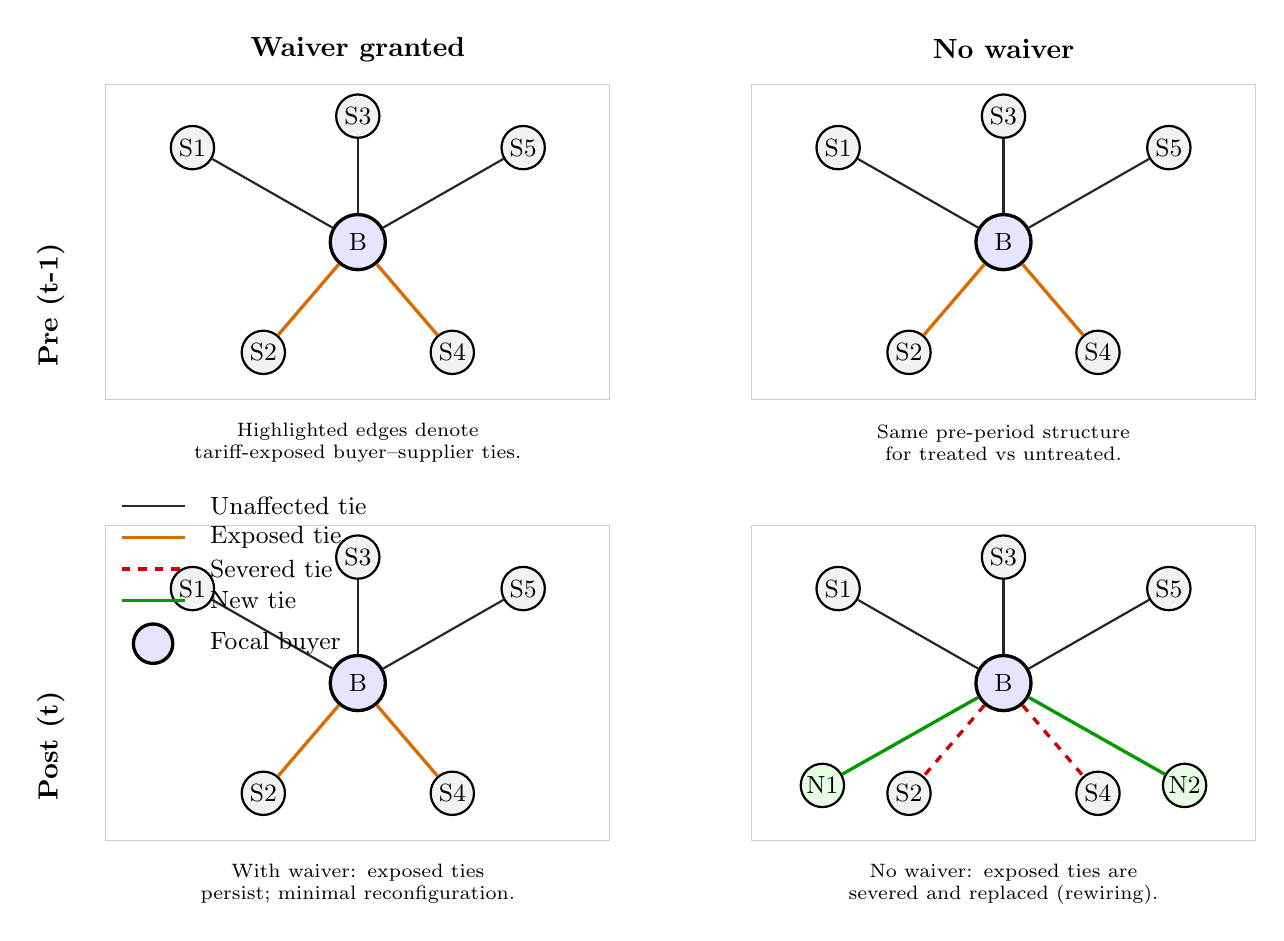
\begin{tikzpicture}[
  >=Latex,
  font=\small,
  % Node styles
  buyer/.style={circle, draw, very thick, fill=blue!10, minimum size=7mm, inner sep=0pt},
  supplier/.style={circle, draw, thick, fill=gray!10, minimum size=5.5mm, inner sep=0pt},
  suppliernew/.style={circle, draw, thick, fill=green!10, minimum size=5.5mm, inner sep=0pt},
  % Edge styles
  tie/.style={thick, draw=black, opacity=0.85},
  affected/.style={very thick, draw=orange!85!black},
  severed/.style={very thick, draw=red!80!black, dashed},
  newtie/.style={very thick, draw=green!60!black},
  paneltitle/.style={font=\bfseries},
  note/.style={font=\scriptsize, align=center, text width=4.2cm}
]

% ------------------------------------------------------------
% Layout: panel anchors (two columns x two rows)
% ------------------------------------------------------------
% Column x Row coordinates
\coordinate (A) at (0,0);      % Waiver, Pre
\coordinate (B) at (8.2,0);    % No waiver, Pre
\coordinate (C) at (0,-5.6);   % Waiver, Post
\coordinate (D) at (8.2,-5.6); % No waiver, Post

% Column headers
\node[paneltitle] at ($(A)+(0,1.45)$) {Waiver granted};
\node[paneltitle] at ($(B)+(0,1.45)$) {No waiver};

% Row headers
\node[paneltitle, rotate=90] at ($(A)+(-3.9,-1.8)$) {Pre (t-1)};
\node[paneltitle, rotate=90] at ($(C)+(-3.9,-1.8)$) {Post (t)};

% Panel boxes (optional)
\draw[gray!40] ($(A)+(-3.2,-3.0)$) rectangle ($(A)+(3.2,1.0)$);
\draw[gray!40] ($(B)+(-3.2,-3.0)$) rectangle ($(B)+(3.2,1.0)$);
\draw[gray!40] ($(C)+(-3.2,-3.0)$) rectangle ($(C)+(3.2,1.0)$);
\draw[gray!40] ($(D)+(-3.2,-3.0)$) rectangle ($(D)+(3.2,1.0)$);

% ------------------------------------------------------------
% Helper macro-ish pattern (done manually to stay simple)
% Each mini-network: one buyer + 5 suppliers around it
% ------------------------------------------------------------

% =========================
% Panel A: Waiver, Pre (t-1)
% =========================
\node[buyer]    (A_b) at ($(A)+(0,-1.0)$) {B};
\node[supplier] (A_s1) at ($(A)+(-2.1,0.2)$) {S1};
\node[supplier] (A_s2) at ($(A)+(-1.2,-2.4)$) {S2};
\node[supplier] (A_s3) at ($(A)+( 0.0,0.6)$) {S3};
\node[supplier] (A_s4) at ($(A)+( 1.2,-2.4)$) {S4};
\node[supplier] (A_s5) at ($(A)+( 2.1,0.2)$) {S5};

% Baseline ties (some highlighted as "affected"/at-risk)
\draw[tie]      (A_b) -- (A_s1);
\draw[affected] (A_b) -- (A_s2);
\draw[tie]      (A_b) -- (A_s3);
\draw[affected] (A_b) -- (A_s4);
\draw[tie]      (A_b) -- (A_s5);

\node[note] at ($(A)+(0,-3.55)$) {Highlighted edges denote\\tariff-exposed buyer--supplier ties.};

% =========================
% Panel C: Waiver, Post (t)
% =========================
\node[buyer]    (C_b) at ($(C)+(0,-1.0)$) {B};
\node[supplier] (C_s1) at ($(C)+(-2.1,0.2)$) {S1};
\node[supplier] (C_s2) at ($(C)+(-1.2,-2.4)$) {S2};
\node[supplier] (C_s3) at ($(C)+( 0.0,0.6)$) {S3};
\node[supplier] (C_s4) at ($(C)+( 1.2,-2.4)$) {S4};
\node[supplier] (C_s5) at ($(C)+( 2.1,0.2)$) {S5};

% With waiver, ego-network is stable (same ties retained)
\draw[tie]      (C_b) -- (C_s1);
\draw[affected] (C_b) -- (C_s2);
\draw[tie]      (C_b) -- (C_s3);
\draw[affected] (C_b) -- (C_s4);
\draw[tie]      (C_b) -- (C_s5);

\node[note] at ($(C)+(0,-3.55)$) {With waiver: exposed ties\\persist; minimal reconfiguration.};

% =========================
% Panel B: No waiver, Pre (t-1)
% =========================
\node[buyer]    (B_b) at ($(B)+(0,-1.0)$) {B};
\node[supplier] (B_s1) at ($(B)+(-2.1,0.2)$) {S1};
\node[supplier] (B_s2) at ($(B)+(-1.2,-2.4)$) {S2};
\node[supplier] (B_s3) at ($(B)+( 0.0,0.6)$) {S3};
\node[supplier] (B_s4) at ($(B)+( 1.2,-2.4)$) {S4};
\node[supplier] (B_s5) at ($(B)+( 2.1,0.2)$) {S5};

\draw[tie]      (B_b) -- (B_s1);
\draw[affected] (B_b) -- (B_s2);
\draw[tie]      (B_b) -- (B_s3);
\draw[affected] (B_b) -- (B_s4);
\draw[tie]      (B_b) -- (B_s5);

\node[note] at ($(B)+(0,-3.55)$) {Same pre-period structure\\for treated vs untreated.};

% =========================
% Panel D: No waiver, Post (t)
% =========================
\node[buyer]      (D_b)  at ($(D)+(0,-1.0)$) {B};
\node[supplier]   (D_s1) at ($(D)+(-2.1,0.2)$) {S1};
\node[supplier]   (D_s3) at ($(D)+( 0.0,0.6)$) {S3};
\node[supplier]   (D_s5) at ($(D)+( 2.1,0.2)$) {S5};

% "Old" suppliers that are severed (kept as nodes for visual continuity)
\node[supplier]   (D_s2old) at ($(D)+(-1.2,-2.4)$) {S2};
\node[supplier]   (D_s4old) at ($(D)+( 1.2,-2.4)$) {S4};

% New suppliers (replacements)
\node[suppliernew] (D_n1) at ($(D)+(-2.3,-2.3)$) {N1};
\node[suppliernew] (D_n2) at ($(D)+( 2.3,-2.3)$) {N2};

% Persisting ties
\draw[tie] (D_b) -- (D_s1);
\draw[tie] (D_b) -- (D_s3);
\draw[tie] (D_b) -- (D_s5);

% Severed exposed ties (red dashed)
\draw[severed] (D_b) -- (D_s2old);
\draw[severed] (D_b) -- (D_s4old);

% New ties (green)
\draw[newtie] (D_b) -- (D_n1);
\draw[newtie] (D_b) -- (D_n2);

\node[note] at ($(D)+(0,-3.55)$) {No waiver: exposed ties are\\severed and replaced (rewiring).};

% ------------------------------------------------------------
% Legend (simple)
% ------------------------------------------------------------
\begin{scope}[shift={($(C)+(-3.0,1.25)$)}]
  \draw[tie] (0,0) -- (0.8,0);       \node[anchor=west] at (1.0,0) {Unaffected tie};
  \draw[affected] (0,-0.4) -- (0.8,-0.4); \node[anchor=west] at (1.0,-0.4) {Exposed tie};
  \draw[severed] (0,-0.8) -- (0.8,-0.8);  \node[anchor=west] at (1.0,-0.8) {Severed tie};
  \draw[newtie] (0,-1.2) -- (0.8,-1.2);   \node[anchor=west] at (1.0,-1.2) {New tie};
  \node[buyer, minimum size=5mm] at (0.4,-1.75) {};
  \node[anchor=west] at (1.0,-1.75) {Focal buyer};
\end{scope}

\end{tikzpicture}
\caption{Ego-network DiD schematic: waiver receipt dampens supplier rewiring.}
\end{figure}
\end{document}

